%1. Final Report: 10 pages + 2 pages on Current Trends in Robotics
%2. Interim Report: 5 pages + 1 page on Current Trends in Robotics
%3. Use latex
%4. Equations describing algorithms must be included.
%5. Analysis plots must be included. (For example, plot error as a function of some experimental parameter such as object distance).
%6. Include an image/photo of the robot
%7. Figures must be your own. No figures can be copied from the web or another periodical (even if it is cited).
%8. Figures must have sufficient captions and be referred to in the text (Using the latex ref command) The figure caption is very important. Discuss the main point of the figure within the caption. Captions are often several sentences.
%9. Label all axes and variables in plots.


%10. For final report: a submission of demo video is required.
%11. Poster is required for department demo day.
%12. Separate from the final report, each person must individually submit a paragraph describing his or her contribution to the project. The tasks of the project should be well distributed (for example, do not have one team member do the all the writing and the other do all the programming).

\documentclass[pdftex,10.5pt]{report}
\usepackage{amsmath}
\usepackage{caption}
\usepackage{graphicx}
\usepackage{import}
\usepackage[hmargin=.97in,vmargin=.97in]{geometry}
\usepackage{hyperref}
\usepackage{cleveref}
\usepackage{multicol}
\usepackage[square,sort,comma,numbers]{natbib}
\usepackage[abs]{overpic}
\usepackage{setspace}
\usepackage{subcaption}
\usepackage{wrapfig}
\usepackage[upright]{fourier} 
\usepackage[usenames,dvipsnames]{xcolor}
\usepackage{tkz-euclide}
\usepackage{listings}
\usepackage{amsmath}

\usetkzobj{all} 
\usepackage{float}
\restylefloat{table}

\renewcommand*\thesection{\arabic{section}}

\makeatletter
\renewcommand\bibsection{
  \section*{\refname
    \@mkboth{\MakeUppercase{\refname}}{\MakeUppercase{\refname}}}
}
\makeatother

\onehalfspacing

\begin{document}

%%%%%%%%%%%%%%%%%%%%%%%%%%%%%%%%%%%%%%%%%
% University Assignment Title Page 
% LaTeX Template
%
% This template has been downloaded from:
% http://www.latextemplates.com
%
% Original author:
% WikiBooks (http://en.wikibooks.org/wiki/LaTeX/Title_Creation)
%%%%%%%%%%%%%%%%%%%%%%%%%%%%%%%%%%%%%%%%%
\begin{titlepage}

\newcommand{\HRule}{\rule{\linewidth}{0.5mm}} % Defines a new command for the horizontal lines, change thickness here

\center % Center everything on the page

%----------------------------------------------------------------------------------------
%	LOGO SECTION
%----------------------------------------------------------------------------------------


\includegraphics{RU_INF_SEAL_CMYK}\\[1cm] % Include a department/university logo - this will require the graphicx package
 
%----------------------------------------------------------------------------------------
 
%----------------------------------------------------------------------------------------
%	HEADING SECTIONS
%----------------------------------------------------------------------------------------

\textsc{\LARGE Rutgers, the State University of New Jersey}\\[1.5cm] % Name of your university/college
\textsc{\Large Senior Capstone Design, Spring '13}\\[0.5cm] % Major heading such as course name
%\textsc{\large Minor Heading}\\[0.5cm] % Minor heading such as course title

%----------------------------------------------------------------------------------------
%	TITLE SECTION
%----------------------------------------------------------------------------------------

\HRule \\[0.4cm]
{ \huge \bfseries Computer Vision-Based 3-D Reconstruction for Object Replication }\\[0.4cm] % Title of your document
\HRule \\[1.5cm]
 
%----------------------------------------------------------------------------------------
%	AUTHOR SECTION
%----------------------------------------------------------------------------------------

\begin{minipage}{0.4\textwidth}
\begin{flushleft} \large
\emph{Authors:}\\
Ryan \textsc{Cullinane}\\
Cady \textsc{Motyka}\\
Elie \textsc{Rosen}
\end{flushleft}
\end{minipage}
~
\begin{minipage}{0.4\textwidth}
\begin{flushright} \large
\emph{Advisor:} \\
Professor Kristin \textsc{Dana} % Supervisor's Name
\end{flushright}
\end{minipage}\\[4cm]


%----------------------------------------------------------------------------------------
%	DATE SECTION
%----------------------------------------------------------------------------------------

{\large \today}\\[3cm] % Date, change the \today to a set date if you want to be precise


\vfill % Fill the rest of the page with whitespace

\end{titlepage}

\begin{abstract}
The Microsoft Kinect for Windows has proven to be a valuable tool in the field of computer vision. The Kinect is comprised of an infrared laser projector and depth sensor. The depth data of a scene is run through a bilateral filter and vector mathematics is used to define the coordinates, connecting lines, the vertices, and edges to form a three-dimensional mesh. The software displays the raw depth data and infrared camera image, this allows the user to filter out objects closer or further than a specified depth, and exports the reconstructed three-dimensional mesh. That mesh is then sliced into horizontal layers and converted into G-Code, a machine language that maneuvers the 3-D printer where to extrude the ABS plastic to create a physical replica of the reconstructed object. 
\end{abstract}

\tableofcontents

\section{Introduction}
% A statement of the problem and its major components in your own words.
The Computer Vision--Based 3-D Reconstruction for Object Replication is accomplished by using a Kinect for Xbox. Originally, the Kinect was created for entertainment, but in recent time, it has been introduced to the field of robotics and computer vision. The Kinect is a quick, reliable, and affordable tool that uses a near-infrared laser pattern projector and an infrared camera, as well as a depth sensor that relays three-dimensional data through the Kinect Software Development Kit (SDK).

The robotics field is beginning to find an increasing number of uses for the 3-D printer. The most innovative aspect of the 3-D printer is the ability to print an object, regardless of interconnecting internal components, and to have it function as intended. For example, any connecting gears that are printed with the 3-D printer will in fact turn as they are supposed to.

\section{Methods}
% A description of how each component in the objective is achieved.
\subsection{Calibration}
The Kinect can be calibrated in a way similar to other cameras for computer vision, the only difference is that changes in the depth have to be present  with the pattern in order to calibrate the depth camera. The Kinect can be calibrated with an image of a checkerboard pattern.

\subsection{Stereo Reconstruction}
Once the Kinect has been calibrated, all that is needed for the stereo reconstruction is a triangulation of viewing rays.

%Depth Disparity Image
\begin{figure}[H]
	\centering
	\begin{tikzpicture}
		\tkzDefPoint(0,0){O_{L}}\tkzDefPoint(6,0){O_{R}}
		\tkzDefPoint(3,4){P}\tkzDefPoint(-.5,.5){leftL}
		\tkzDefPoint(1.5,.5){leftR}\tkzDefPoint(4.5,.5){rightL}
		\tkzDefPoint(6.5,.5){rightR}\tkzDefPoint(3,0){B}
		\tkzDefPoint(3,.5){A}
		\tkzDefPoint(.38,.5){P_{L}}
		\tkzDefPoint(5.6,.5){P_{R}}
		\tkzDrawSegments(O_{L},P P,O_{R} O_{R},O_{L} leftL,leftR rightL,rightR B,P)
		\tkzDrawPoint(A)
		\tkzDrawPoint(B)
		\tkzDrawPoint(P_{L})
		\tkzDrawPoint(P_{R})
		\tkzLabelPoints[below](O_{L},O_{R})
		\tkzLabelPoints[above](P)
		\tkzLabelPoints[above left](P_{L})
		\tkzLabelPoints[above right](P_{R})
		\tkzLabelPoints[above right](A)
		\tkzLabelPoints[below right](B)
	\end{tikzpicture}
	\caption{Visual Representation of Depth Disparity.}
\end{figure}

P is the location of the object in the world, $O_{L}$ and $O_{R}$ are the left and right camera centers, $P_{R}$ and $P_{L}$ are the appearance of the point P in the two image planes where, 
\begin{figure}[H]
	\centering
	 $P_{L}= 
	\begin{bmatrix}
		x_{L} \\
		y_{L} 
	\end{bmatrix}$.
\end{figure}
The distance between $O_{L}$ and $O_{R}$ is T, the distance between the left and right camera. The distance between A and B is the focal length of each of the cameras. If the distance between P and B is defined as distance Z, the following equation  can be used to represent the ratio between T and Z, using the theorem of like triangles,
\begin{figure}[H]
	\centering
	$\frac{T}{Z}=\frac{T+x_{L}-x_{R}}{Z-f} or \frac{T-{x_{R}-x_{L}}}{Z-f}$. 
\end{figure} 
Cross multiplying these equations results in,
\begin{figure}[H]
	\centering
	$\frac{Z(T-x_{R}-x_{L})}{Z-f} = \frac{T(Z-f)}{Z}$. 
\end{figure}
These calculations show that depth, Z, is inversely proportional to the disparity. Therefore,  
\begin{figure}[H]
	\centering
	$P_{L}= \frac{f^{L}P}{Z_{L}} $ and $P_{R}= \frac{f^{R}P}{Z_{R}}.$
\end{figure} 

Once there is a corresponding point pair for P from the two images, an algorithm would undo the scale and shift of the pixel points in order to obtain two-dimensional camera coordinates. The midpoint algorithm is then used to find the actual three-dimensional world coordinate that corresponds to that point pair.

%Midpoint Algorithm Image
\begin{figure}[H]
	\centering
	\begin{tikzpicture}
		\tkzDefPoint(0,0){p_{L}}\tkzDefPoint(6,0){p_{R}}
		\tkzDefPoint(3,3){p_{a}}\tkzDefPoint(3,2){p_{b}}
		\tkzDefPoint(3,2.5){P}
		\tkzDrawSegments(p_{L},p_{b} p_{a},p_{b} p_{R},p_{a})
		\tkzDrawPoint(P)
		\tkzDrawPoint(p_{L})
		\tkzDrawPoint(p_{R})
		\tkzDrawPoint(p_{a})
		\tkzDrawPoint(p_{b})
		\tkzLabelPoints[above left](P)
		\tkzLabelPoints[above left](p_{a})
		\tkzLabelPoints[above right](p_{b})
		\tkzLabelPoints[above right](p_{R})
		\tkzLabelPoints[above left](p_{L})
	\end{tikzpicture}
	\caption{Visual Representation of the Midpoint Algorithm.}
\end{figure}

Above are the rays $\vec{O_{R}p_{R}}$ and $\vec{O_{L}p_{L}}$. The line connecting the two vectors, perpendicular to both, is obtained by taking the cross product of these two vectors. The vector,

\begin{figure}[H]
	\centering
	 $\vec{p_{L}p_{b}} = a\vec{p_{L}}$, 
\end{figure}	 

\noindent and since point $p_{R}$ is distance T away from $p_{L}$, 

\begin{figure}[H]
	\centering
	$\vec{p_{R}p_{a}} = b^{L}R_{R}\vec{p_{R}}+T$. 
\end{figure}	

\noindent The segment connecting these two vectors can be represented as,

\begin{figure}[H]
	\centering
	$\vec{p_{a}p_{b}} = c\vec{p_{L}}x^{L}R_{R}\vec{p_{R}}$,
\end{figure}

\noindent where $a,b,$ and $c$ are unknown constants that can be solved using the three aforementioned equations. The point P lies on the center of this line and is found where,

\begin{figure}[H]
	\centering
 	$^{L}P=a\vec{p_{L}}+\frac{c}{2}\vec{p_{L}}x^{L}R_{R}\vec{p_{R}}$.
 \end{figure}

\noindent In order to get the world point M, $^{L}P$ would is divided by the intrinsic and extrinsic matrices of the Kinect.

% How Kinect does triangulation 
\begin{figure}[H]
	\centering
	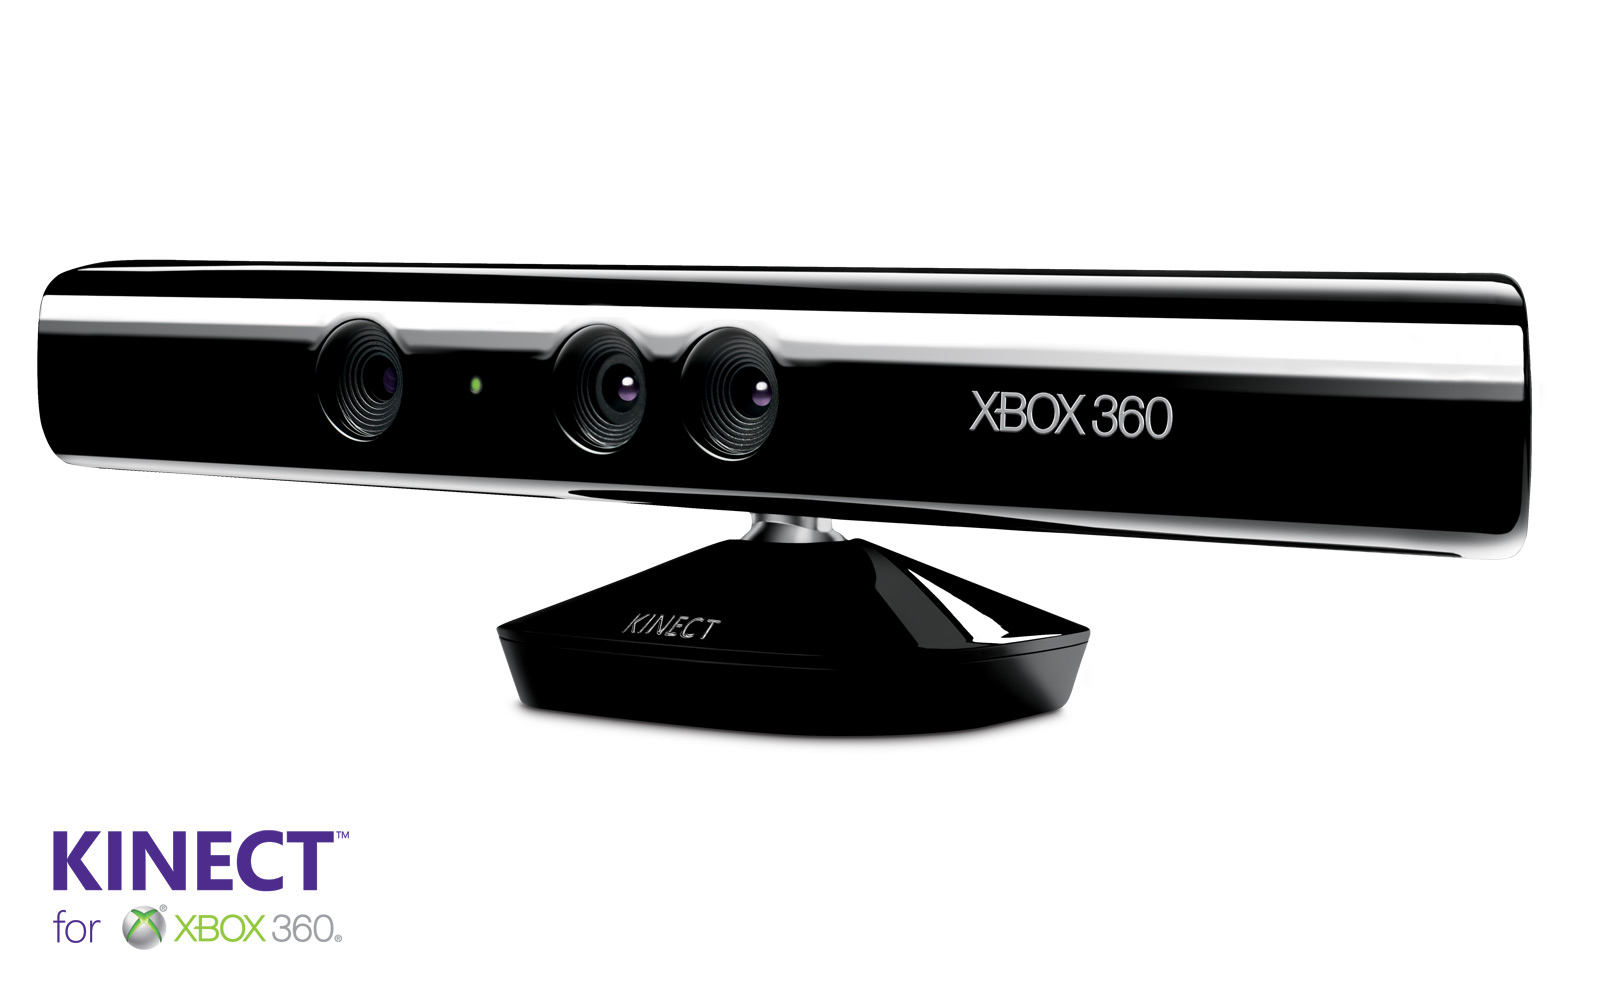
\includegraphics[width=70mm]{figures/kinect.jpg}
	\caption{The Kinect for Xbox. The hole on the left is an infrared light source, the center is a RGB camera, and the three-dimensional depth sensor is on the right. In addition to these cameras, the base has a motorized tilt and a multi-array microphone that goes along the bottom of the device.}
	\label{kinectlable}
\end{figure}

The Kinect accomplishes triangulation by using the known information about the sensor, the data obtained from the infrared projection, and the image received from the camera. The sensor projects infrared light onto an object, the light then bounces back, and the infrared sensor reads in the data from the reflected light. These clusters of captured light can be matched to the hard-coded images the Kinect has of the normal projected pattern, and allows for a search for correlations, or the matching points. While looking through the camera's focal point, the point of interest will fall on a specific pixel, depending on how close or far away it is, providing the end point for the trajectories coming from the camera and projector. These relative lines of trajectories, along with the known information about the distance between the cameras on the Kinect sensor, are used in the triangulation process to find the three-dimensional coordinates of the point. Figure ~\ref{kinectlable} the sensor arrangement of the Kinect for Xbox.

\subsection{Bilateral Filter}
In order to make the depth data cleaner and less noisy, a bilateral filter is used to remove the erroneous measurements. The bilateral filter takes the depth at every point, and recalculate the depth value at that point based on a waited average of the surrounding pixels in a specified neighborhood. The process takes away some of the sharpness of the depth map, but it removes the noise that skews the results of the three-dimensional reconstruction. The filter follows a Gaussian approach which calculate a new depth at every depth pixel in the image and replaces it with,
\begin{figure}[H]
	\centering
	$BF[I]_{P} = \frac{1}{16} \left( 
	\begin{array}{ccc}
		1 & 2 & 1 \\
		2 & 4 & 2 \\
		1 & 2 & 1 
	\end{array}  \right)$,
\end{figure}
\noindent multiplied by the neighborhood of the three by three square of pixels around the pixel that is being changed. The resulting depth value represents the average of the nine pixels, where the closer pixels weights in the average are heavier than the further pixel values' weights.  \cite{filter}

\subsection{Mesh Construction}
Once the depth data has been filtered, it can be used to create a three-dimensional mesh of the object. At each pixel location two vectors are made, each connecting that three-dimensional point to both the neighboring point to the right and below. Figure ~\ref{square} shows the square that is is looked at for each x and y coordinate. Cross multiplying the two vectors of adjacent sides results in the orientation vector for the point or its normal vector. As the loop goes through each point, it creates a triangle in three-dimensional space out of the existing points and calculated orientations, which are recorded in three-dimensional point and vector collections. Figure ~\ref{triangle} shows the recorded three-dimensional point, normal vectors and orientation of that triangle in the mesh. Each of these points must be added in the correct order, keeping with the right hand rule, so that each reconstructed triangle is oriented in the correct direction. While these three points and vectors are added, separate collections of the indicies and texture information are recorded. 

%Mesh square
\begin{figure}[H]
\centering
	\begin{tikzpicture}
		\tkzDefPoint(0,3){p_{1}}\tkzDefPoint(3,3){p_{2}}
		\tkzDefPoint(0,0){p_{3}}\tkzDefPoint(3,0){p_{4}}
		\tkzDrawSegments(p_{1},p_{2} p_{2},p_{4} p_{3},p_{4}  p_{1},p_{3} p_{2},p_{3})
		\tkzDrawPoint(p_{1})
		\tkzDrawPoint(p_{2})
		\tkzDrawPoint(p_{3})
		\tkzDrawPoint(p_{4})
		\tkzLabelPoints[above left](p_{1})
		\tkzLabelPoints[above right](p_{2})
		\tkzLabelPoints[below left](p_{3})
		\tkzLabelPoints[below right](p_{4})
	\end{tikzpicture}
	\caption{The square used to build the three-dimensional mesh}
		\label{square}
\end{figure}

While reconstructing the front face of the mesh, our algorithm goes through every x and y pixel coordinate starting at (0,0) and ending with (320,240), incrementing by a scale factor number that can be adjusted for less demand on the computers processor. Down sampling for testing was accomplished by setting the number to two so that only every other point was processed. In the software the user can also crop out the left, right, top or bottom of the image. Changing these sliders indicates where on the image the reconstruction of the mesh is going to begin and end. The user can also specify what they would like the minimum and maximum depth to be. 

%Mesh Triangle
\begin{figure}[H]
\centering
	\begin{tikzpicture}
		\tkzDefPoint(0,3){p_{1}}\tkzDefPoint(3,4){p_{2}}
		\tkzDefPoint(1,1){p_{3}}\tkzDefPoint(1.5,2.5){A}
		\tkzDefPoint(4.5,4){B}\tkzDefPoint(2.5,.5.5){C}
		\tkzDrawSegments(p_{1},p_{2} p_{2},p_{3} p_{3},p_{1})
		\tkzDrawPoint(p_{1})
		\tkzDrawPoint(p_{2})
		\tkzDrawPoint(p_{3})
		\tkzLabelPoints[above left](p_{1})
		\tkzLabelPoints[above left](p_{2})
		\tkzLabelPoints[below left](p_{3})
		\draw [-latex, thick, shorten >= 1.00cm] (p_{1}) -- (A);
		\draw [-latex, thick, shorten >= 1.00cm] (p_{2}) -- (B);
		\draw [-latex, thick, shorten >= 1.00cm] (p_{3}) -- (C);
	\end{tikzpicture}
	\caption{The correctly oriented triangle of the three-dimensional mesh}
	\label{triangle}
\end{figure}

In order to filter out depth that is further than the intended value, the software looks at the square where the point of interest is the upper left corner.  If all four points are outside of the depth range, that point is skipped. If any of the four points on that square are within the depth range, the square is constructed. For the square, any point that is not within the depth range is given the depth of the back wall, the value specified by the user. Lastly, the back wall of the three-dimensional reconstruction is built. A loop goes through every point that is already in the three-dimensional point collection and each point is copied to the end of the collection with the depth changed to the depth of the back wall. The same number of orientation vectors are added to the collection of three-dimensional vectors, each one equaling [0,0,-1]. 
\cite{cite8}

% G-code Conversion
\subsection{G-code Conversion}
The RepRap 3-D printer firmware uses G-code to communicate to the 3-D printer, specifically to define the print head movements. G-code has commands that tell the print head to move to a certain point with rapid or controlled movement, turn on a cooling fan, or select a different extruding tool. Since the RepRap 3-D printer does not have as many features, the G-code generator does not have to add much extra complicated code, but rather only instructions to the printer head and to turn on the heating elements. Since the printer continuously dispenses plastic, it is necessary to find a path for it to take that will build up the reconstructed object layer by layer without placing too much plastic in any specific area. The conversion requires cutting up the reconstructed object into layers and then finding the best path to traverse that layer without overlapping any part of that path. The G-code converter takes in a STL file, cuts it up into horizontal layers, and then calculates the amount of material that is needed to fill each slice. All this is taken care of by the Slic3r project created by Alessandro Ranellucci. \cite{slic3r} An attempt was made to create the converter within the scope of the semester project, however, it was determined that this alone might have taken the whole semester. 

%3-D printer
\subsection{Building a 3-D Printer}
The RepRap Prusa Mendel Iteration 2 is nothing more than "an inventory of parts" which lists all of the necessary components and design files for building the printer from scratch. A non-exhaustive list of components include; threaded metal rods, linear bearings, nuts, screws, washers, and electrical heating elements. \cite{reprap} These parts were purchased from A2APrinter located in Toronto, Canada and arrived by early February. Once the printer arrived, work began to meticulously build the kit following the poorly written specified instructions. In all, there are over 100 pieces to make the printer and each fit in custom 3-D printed parts that were extruded using a secondary MakerBot Replicator 2 3-D printer owned by the  Institute of Electrical and Electronics Engineers (IEEE) Princeton Central Jersey Section. The final printer includes a heated extruder nozzle that heats up to 400 degrees Fahrenheit to melt the ABS plastic and a heating bed which heats up to about 200 degrees Fahrenheit to keep the printing object soft and malleable as to allow the completed object to cool evenly since the plastic shrinks minimally when cooling and would cause defiguration in the final printed object.

\section{Experimental Results}
%Measurements, repeated trials (for validation), error/performance analysis (as a function of system parameters). Include plots, images or tables to describe measurement values.
%Figure 4 blurb
To obtain an initial grasp of how the Kinect captures data from a three-dimensional scene precompiled demo programs included in the Helix 3D Toolkit were examined. \cite{helix} Figure ~\ref{waterbot}  shows the initial tests done using the Helix Kinect Demo which allows the user to control the angle of the Kinect along with other built in settings. This program records the depth data from the infrared depth sensor and maps the color data from the RGB camera to the corresponding points on the depth image to recreate a three-dimensional scene. As can be seen in the figure, the data is very rough and contains a significant amount of missing data causing empty space when viewing the recreation from certain angles. This is due to the fact that only one image of the scene is used and has no methods to obtain information for objects hidden behind closer objects in the scene.

\begin{figure}[H]
	\centering
	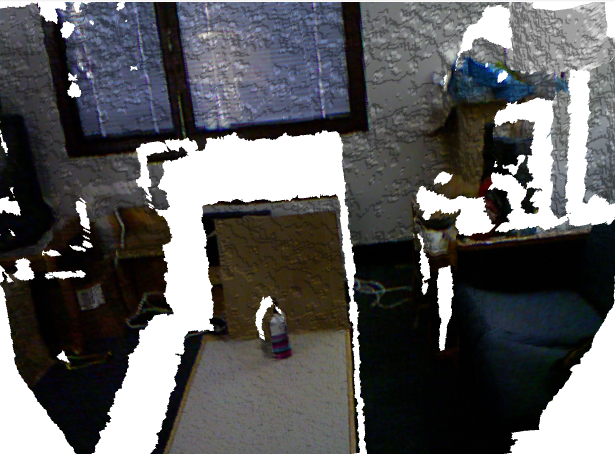
\includegraphics[width=70mm]{figures/kinectwaterbottle.png}
	\caption{Kinect raw depth data with RGB image mapped to it. It is also important to notice the lack of filtering to smooth the data.}
	\label{waterbot}
\end{figure}

%Figure 5 blurb
The next step moving forward was to transform this data into a three-dimensional mesh. The basic primitive of a three-dimensional mesh is a polygon, in this case a triangle, which when linked with other polygons creates a contoured surface to represent the object. This representation was initially achieved by creating single triangles at each depth data, which scaled in size depending on the point's distance relative to the Kinect camera as seen in Figure ~\ref{3dtri}. Using this representation as a starting platform, it was quickly determined that much of the data would not contribute to the construction of the model and could therefore be discarded. To achieve this, near and far data filters were applied to the data sets which would eliminate anything closer or further than the set values of the near and far filters respectively.

\begin{figure}[H]
	\centering
	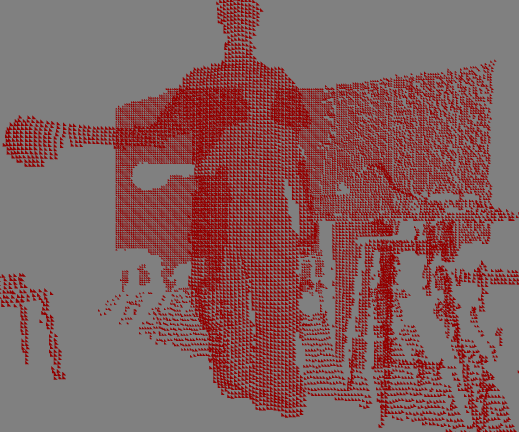
\includegraphics[width=70mm]{figures/3dtriangles.png}
	\caption{Triangles representing the three-dimensional data.}
	\label{3dtri}
\end{figure}

%Figure 6 blurb
With near and far depth filters in place, the excess data is removed from the three-dimensional representation which was referred to as the "3-D mesh" at that stage of the project. A significantly cleaner mesh can be seen in Figure ~\ref{balls2}, where all but the subject of the image is excluded, removing the unwanted objects such as the chairs, tables, and wall that can be seen in the infrared depth image in the upper right hand corner. This stage of the 3-D mesh still contained missing data which caused discontinuities in the mesh which would not allow for the mesh to be a printable object. These "holes" would be addressed at a later stage when a more accurate representation of the mesh could be obtained.

\begin{figure}[H]
	\centering
	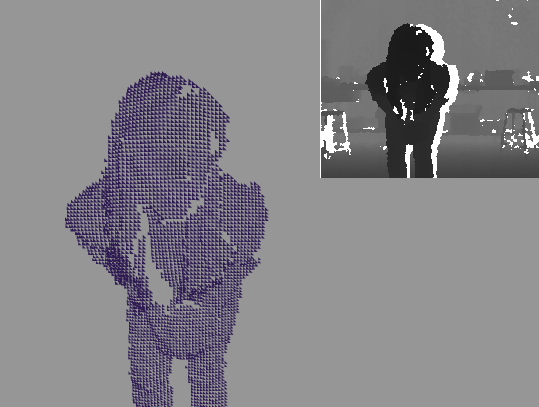
\includegraphics[width=70mm]{figures/cadyholdingball2.png}
	\caption{Comparison of depth frame data with background filtered out.}
	\label{balls2}
\end{figure}

It was determined after initial trials with the software that by not filtering the depth data, the final mesh had a lot of noise which made the figure unpleasant to observe. By implementing a Gaussian-based Bilateral Filter, the results improved significantly and provided an elegant and clean model that could then be printed. This process can best be seen in Figure ~\ref{fig:filtering}.

\begin{figure}[H]
	\centering
	\begin{subfigure}[H]{0.4\textwidth}
		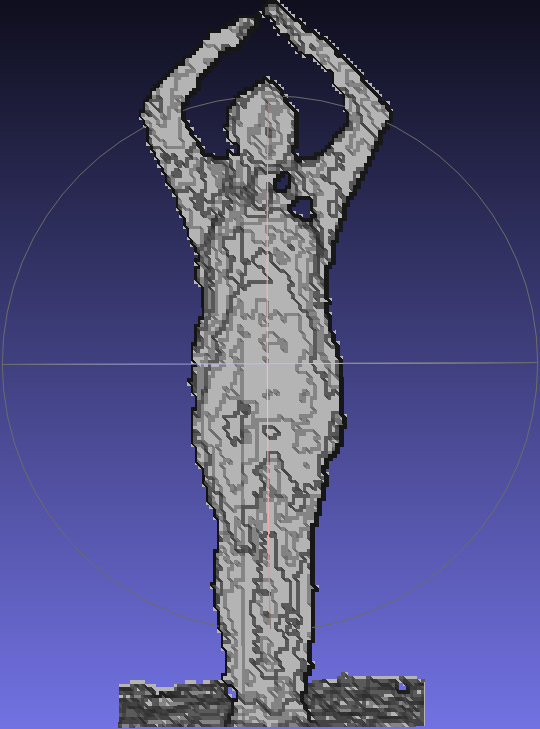
\includegraphics[width=\textwidth]{figures/unfiltered}
		\caption{Non-filtered scan}
	\end{subfigure}
	\begin{subfigure}[H]{0.4\textwidth}
		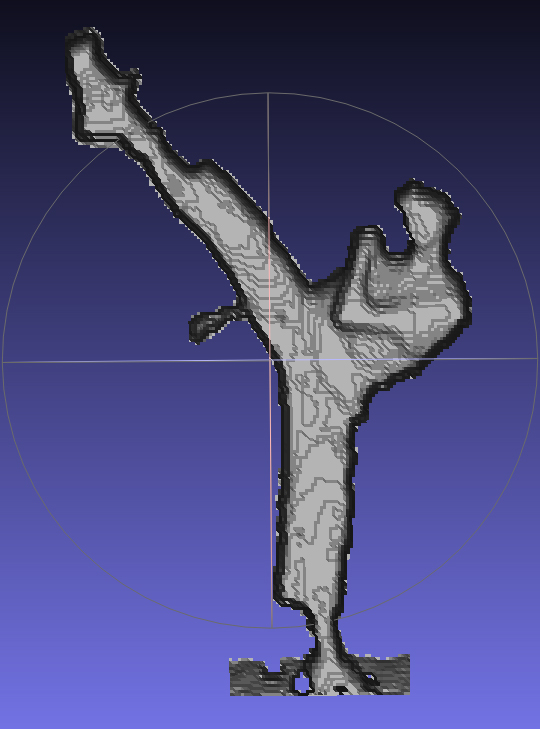
\includegraphics[width=\textwidth]{figures/filter}
		\caption{Gaussian filtered scan}
	\end{subfigure}
	\caption{As can be seen on the right figure it is clear that filtering the depth data provides 
		a nicer, cleaner, and smoother result.
	}
	\label{fig:filtering}
\end{figure}

Through all these trial and error steps a final product of miniature figurines was achieved as can be seen in Figure ~\ref{fig:actionfigures}. These figurines were created by scanning the project creators in various poses, then exporting the meshes and creating the machine language G-code which is read by the printer. The final printed object is 20\% of the original exported mesh and additionally 100 times smaller from the original depth data, the printed objects are about 50mm tall and on average takes between 20 - 30 minutes to print each one.

\begin{figure}[H]
	\centering
	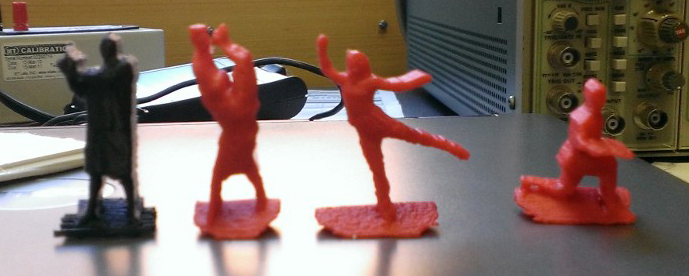
\includegraphics[width=70mm]{figures/actionfigures.jpg}
	\caption{Final result - 3-D printed objects that were scanned through the KinectScan application.}
	\label{fig:actionfigures}
\end{figure}

To check the accuracy of the three-dimensional models versus real world height, Ryan held a tape measure above his head which came out to approximately 213.36 cm. A height measurement was also performed in the 3-D model software which came out to 210.257 cm. The process can be seen in Figure ~\ref{fig:sizes} and comes out to a 1.45\% error which shows that the scan is fairly accurate in correctly representing scale and detail.

\begin{figure}[H]
	\centering
	\begin{subfigure}[H]{0.4\textwidth}
		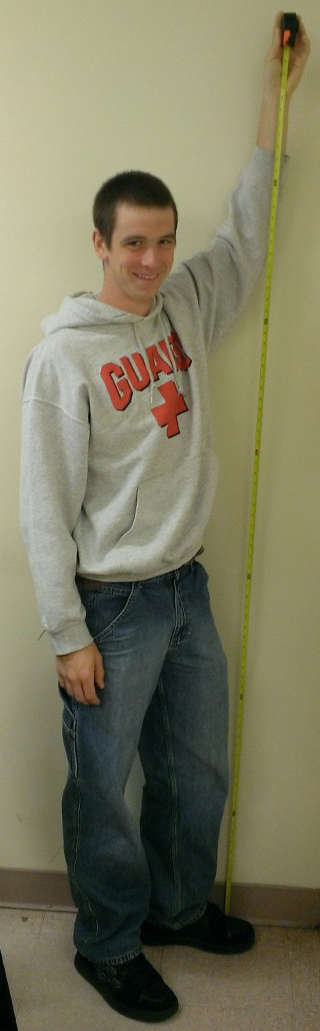
\includegraphics[height=108mm, width=40mm]{figures/ryanmeasure}
		\caption{Actual Height - 7 ft or 213.36 cm}
	\end{subfigure}
	\begin{subfigure}[H]{0.4\textwidth}
		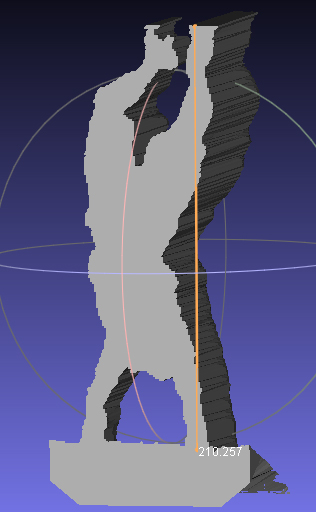
\includegraphics[width=\textwidth]{figures/ryanhandstandmeasure}
		\caption{3-D mesh - 6.81 ft or 210.257 cm}
	\end{subfigure}
	\caption{Comparison between actual and modeled height, the results are very close.}
	\label{fig:sizes}
\end{figure}

\section{Discussion}
%Discuss difficulties, sources of error, future work and extensions.
An issue with the RepRap 3-D printer is that many of the parts used in the construction of the machine are printed by another 3-D printer. Therefore, we had to wait for all of the correct parts to be printed before we could finish construction of our printer. We discovered that two important parts were missing and therefore we had to go to the Rutgers Maker Space to get these parts printed. The only problem we found with the printed parts was that the holes in the plastic were the exact diameter of the rods that were supposed to fit in. Since forcing the rods into place might have placed too much stress on the plastic parts, we use hot water to make the printed plastic more malleable.

Another issue with the construction of the 3-D printer was the lack of good documentation on the assembly process. The triangular base structure had to be taken apart and reassembled multiple times in order to fix errors. One example was the motor bracket for the motor that controls the movement along the y-axis: there were no diagrams good enough to show which side of the machine the part should be placed and what direction it should be oriented. Figure~\ref{parts} shows a number of the unlabeled parts that we received from the IEEE. Since documentation was hard to find and none of the parts were labeled, we also had trouble finding the correct STL files to send to get printed. We knew that we were missing the brackets that connect the two top motors to the threaded rod that controls the movement along the z-axis, but we did not know exactly what file needed to be printed.

\begin{figure}[H]
	\centering
	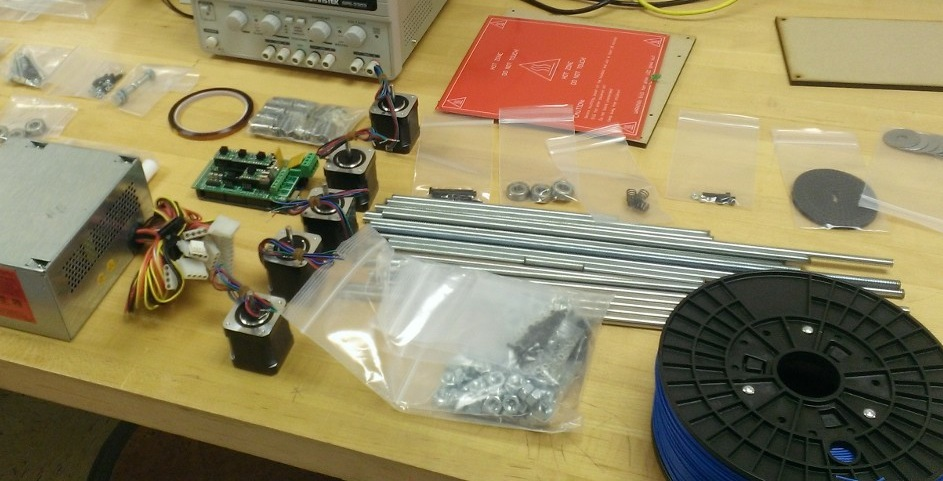
\includegraphics[width=70mm]{figures/WP_20130223_002.jpg}
	\caption{Parts of the 3-D  Printer.}
	\label{parts}
\end{figure}

Even after the mechanical parts of the 3-D printer had been constructed, we still needed to calibrate all of the axes, add all of the electrical components, calibrate the firmware, and build the protective frame around the printer. Figure ~\ref{basebuilt} shows the constructed frame, x,y, and z-axes and the installed printer. One of the issues that we were faced with as we completed the 3-D printer was with the extruder. The extruding component is responsible for heating and melting the Acrylonitrile Butadiene Styrene (ABS) plastic and placing it onto the right spot on the heat bed. We discovered a problem in using normal solder since it could not handle the heat that was needed to melt the ABS plastic. As a result, the piece fell apart as the machine heated up. In order to fix the melting issue, we had to order silver solder since it is capable of withstanding 221 degrees Fahrenheit.

\begin{figure}[H]
	\centering
	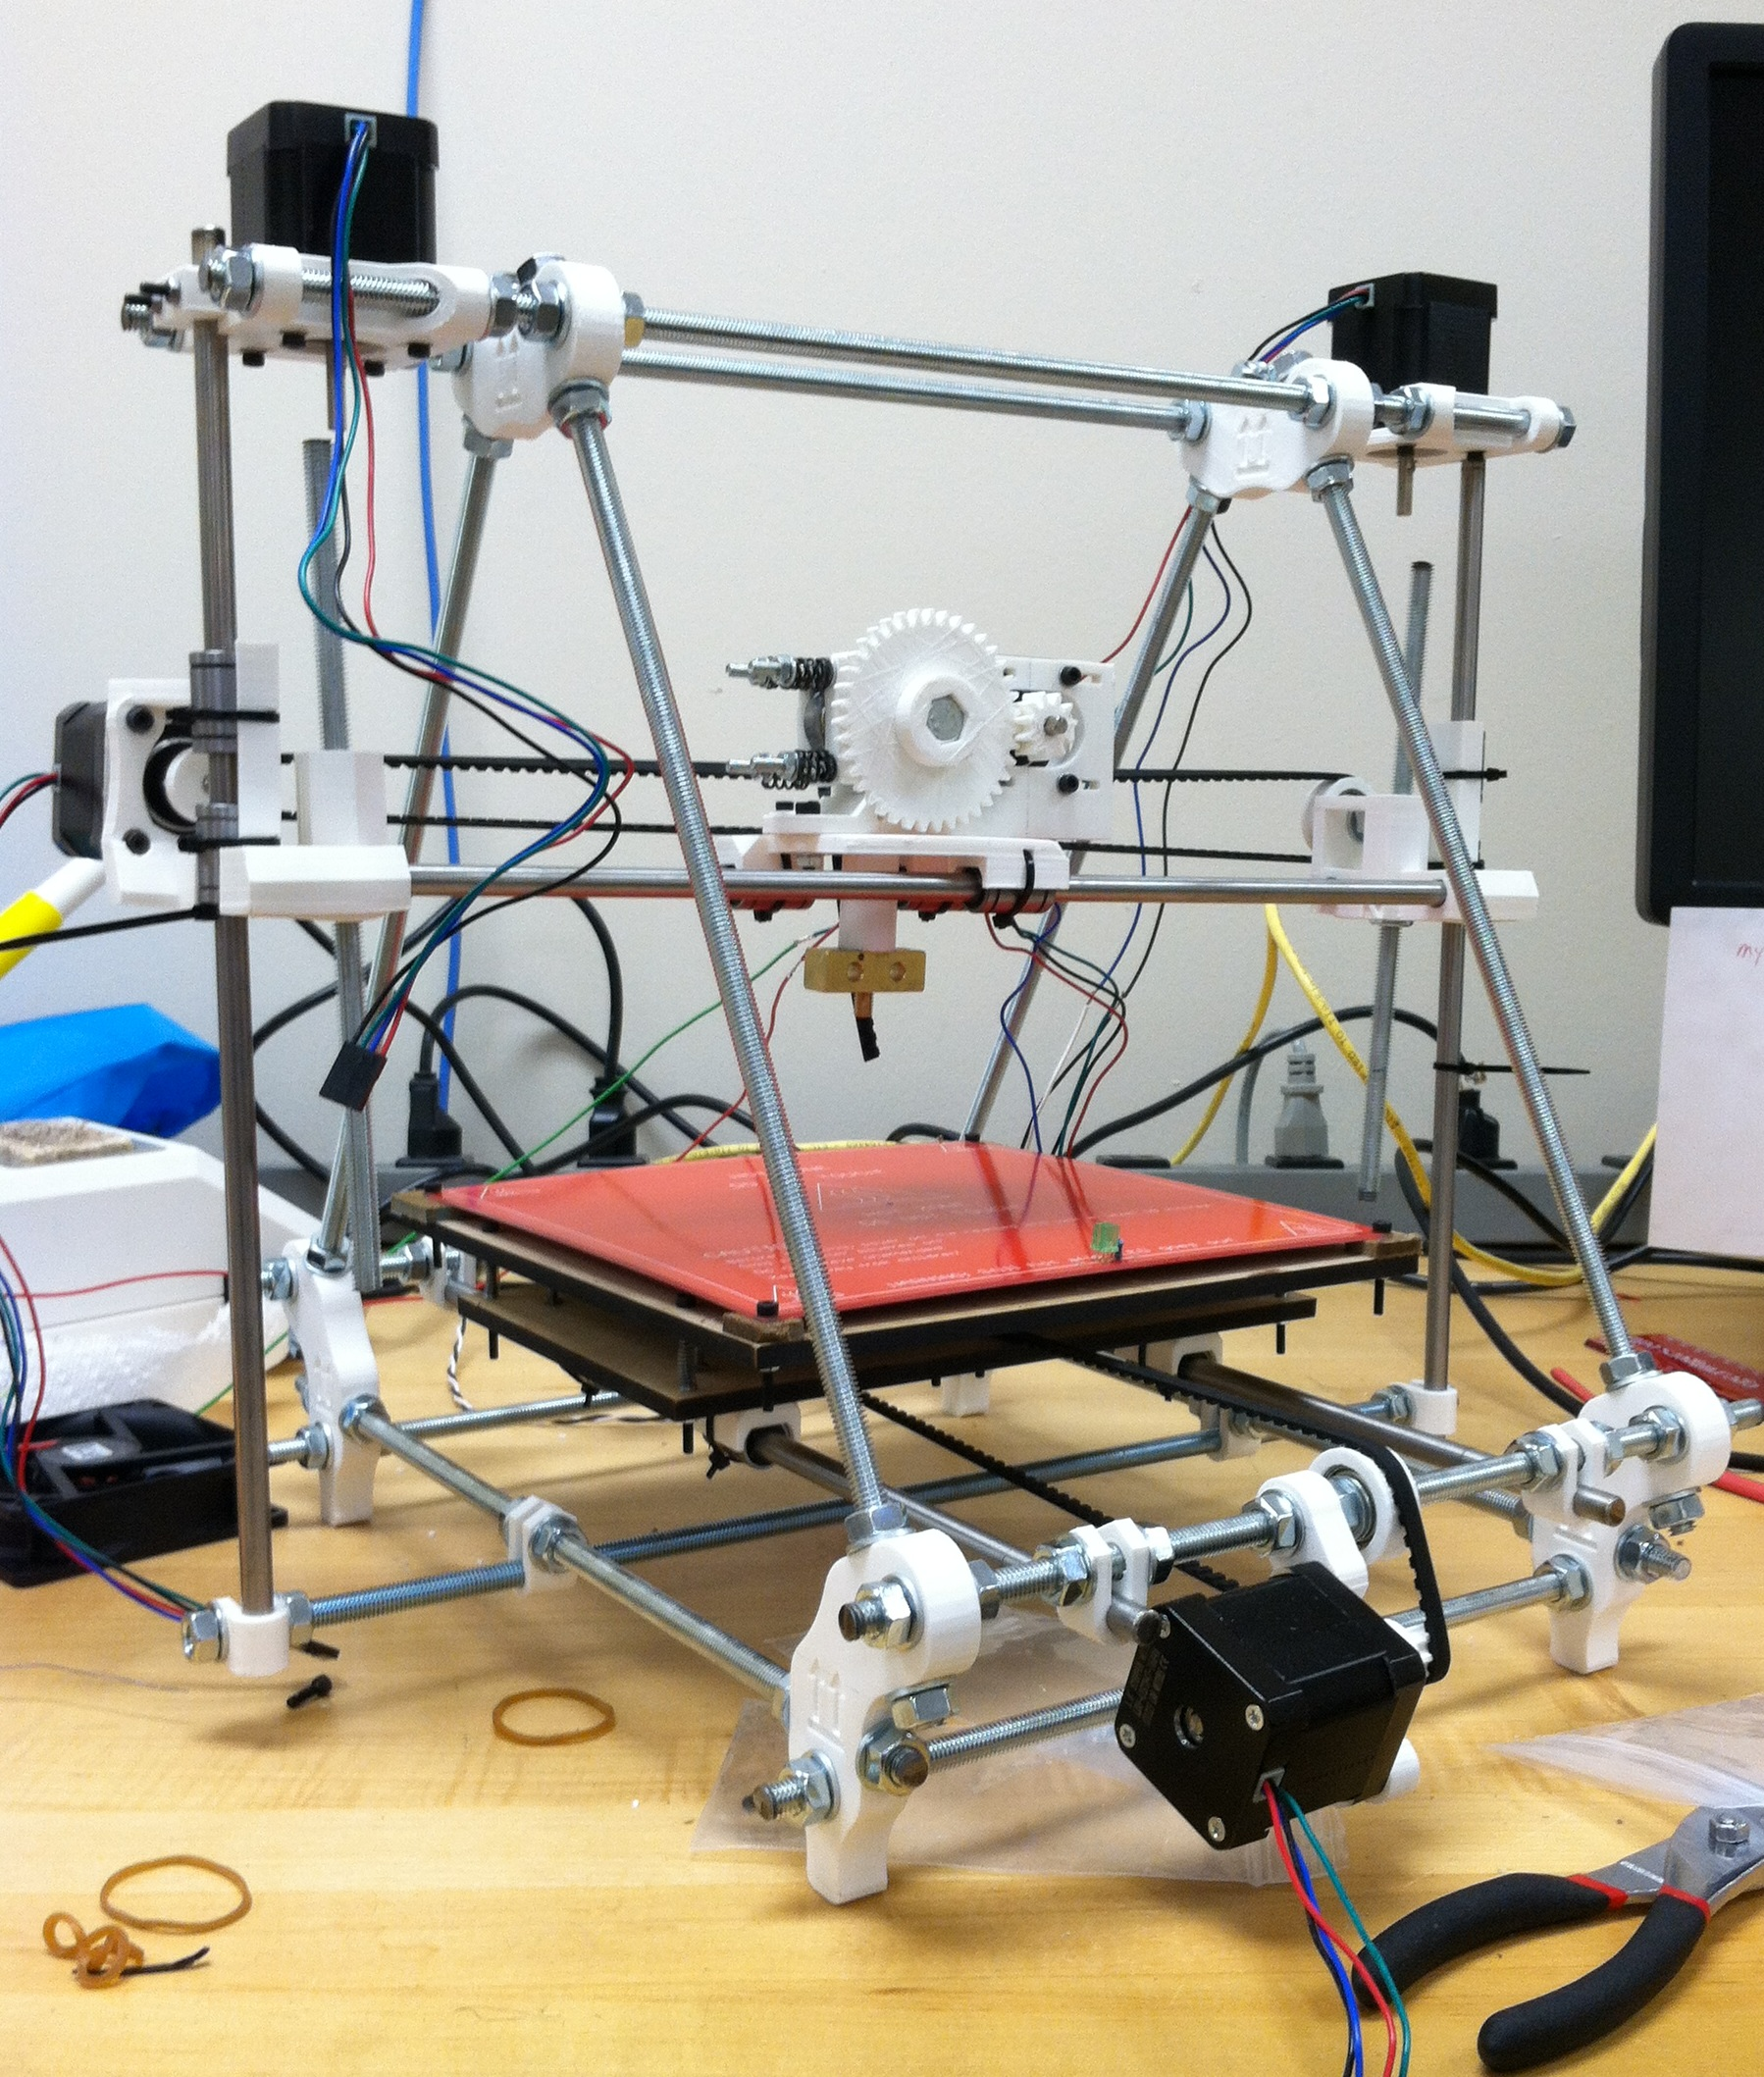
\includegraphics[width=70mm]{figures/photo.JPG}
	\caption{Construction of the 3-D Printer Frame and x,y, and z-axes.}
	\label{basebuilt}
\end{figure}

The biggest problem that we experienced with the software component of the project was the lack of examples and demo code to work with. Other people who have worked on similar projects used the original version of the Microsoft Kinect SDK before its official release so many demo implementations required packages that are no longer part of the latest version of the SDK. Instead, we had to find ways to make them work the new SDK, which was released in 2012, and works in a way similar to the old SDK.

Since our application uses the infrared sensor, the scan will not come out at intended under a few conditions. When outside the Kinect cannot collect the data as well as it can inside. At Rutgers Day an all day open house event at Rutgers, we notice that when people stood below the sky light there was essentially no data being collected at the top of their heads because of the sunlight. In addition, our application is dependent on the reflectivity of the object that it is scanning. For example, if someone holds a clear plastic cup in front of their body during the scan, it may appear as if there is a hole in that person's body because the Kinect is unable to record depth data in that area.

\begin{figure}[H]
	\centering
	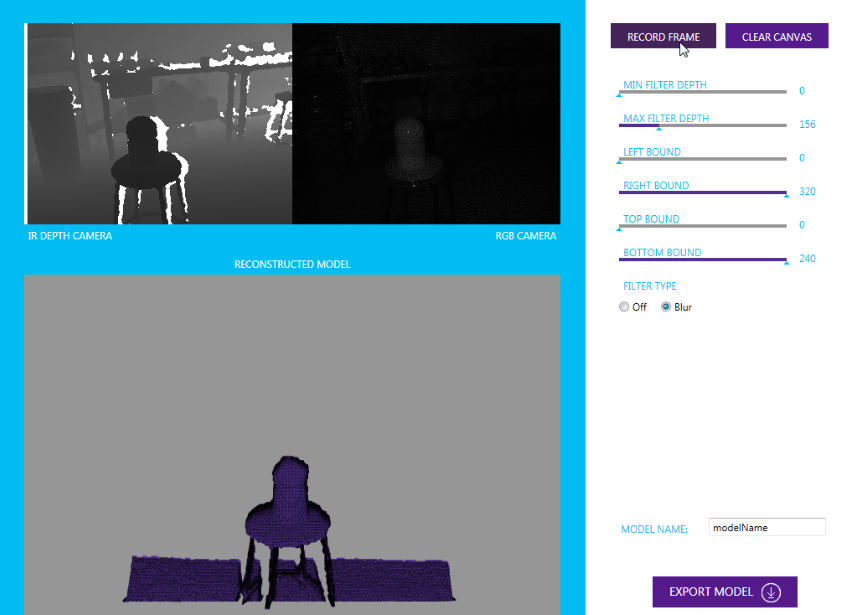
\includegraphics[width=70mm]{figures/KinectScan.jpg}
	\caption{Custom application designed to create three-dimensional meshes - KinectScan}
	\label{kinectscan}
\end{figure}

The final version of our custom application, KinecScan, is shown in Figure \ref{kinecrscan}. The upper left image is a grayscale representation of the depth data that the Kinect is receiving, closer objects are darker in color than objects further away, white indicates that there is no depth data for that pixel. The right image is the RGB camera video feed but set to infrared mode to show the infrared dot matrix. Both of these video streams allow the user to have a good idea of what information will be used to construct the mesh of the current scene. With this application, the user can specify the maximum and minimum x, y and depth values. Adjusting the maximum depth will filter out the background and reconstruct only the object as shown in Figure \ref{kinectscan}. The x and y filters are useful to crop the window if there is some unmovable object next to the item desired to be scanned, like a column or wall, that is close enough that the depth filer can not filter it out. There is also an option provided to turn the bilateral filter on or off. The two buttons on the top allow the user to record the frame; once this is selected, the three-dimensional reconstructed mesh would appear in the bottom gray window. The button in the upper right corner will clear the canvas and all of the information used to make the three-dimensional mesh. The field at the bottom is used to indicate what the file name will be when the user presses the button at the bottom of the application, that exports the model with the file name specified above it.

\section{Cost Analysis}
%Discuss the cost entailed with a product design based on your work. Use examples from currently available equipment in your cost estimates.
The project in itself is not by any means cost effective in that there is a large cost alone in acquiring a 3-D printer. The printer used in this project costs a little over \$550.00 which is not representative of the true expense of large professional 3-D printers; which can cost into the thousands of dollars. Work is currently being performed in industry to lower this cost in order to make it affordable so that even regular consumers may purchase 3-D printers for their homes. \cite{cite9} The printer however, was payed for through a grant with the IEEE Princeton Central Jersey Section so there was no direct cost to the project. 

Other components to the project included a Microsoft Kinect for Xbox which performed 3-D scanning. The cost for this powerful sensor is about\$100.00 which for the hardware included is a great price and opens the use of 3-D sensing to just about any project one can think of. The rest of the miscellaneous parts purchased for this project include acrylic casing to make the project more professional. Additional Pololu stepper motor drivers where purchased due to the malfunctioning of the drivers which originally came with the printer kit. A full list of parts used and their costs can be found in Table ~\ref{tab:costs}.

\begin{table}[H]
	\centering
 	\begin{tabular}{|l|c|c|}
		\hline
		\textbf{Item} & \textbf{Description} & \textbf{Cost} \\
		\hline
 		RepRap Prusa Mendel Iteration 2 & Open Hardware based 3-D Printer& \$ 556.03\\
		Microsoft Kinect for Xbox & Video camera and depth sensor & \$ 98.79 \\
		Acrylic casing, small tools, glue, misc.. & Parts for creating the case & \$ 59.65 \\
		Pololu A4988 Stepper Motor Driver ($\times 3$)   & Converts digital signals to motor movement & \$ 33.09 \\
		Kinect Power Supply Cable & External power source for Kinect & \$ 6.70 \\
		\hline
		& \textbf{Total Cost:} & \textbf{\$  754.26} \\
		\hline
	\end{tabular}
	\caption{
	Overview of hardware and cost for project.
	}	
\label{tab:costs}
\end{table}

\section{Current Trends in Robotics and Computer Vision}
% Describe real world robotic systems of research programs that are related to your capstone project. Research the literature and provide formal citations from publications (as obtained from IEEE Xplore or ACM Digital Library on the Rutgers library site) and periodicals (e.g. NY Times, Wall Street Journal). Do not use websites as sources for this section.

\subsection{Kinect Revolution}
One of the reasons that the Kinect has become so popular for computer vision projects is that it is cheap, quick, and highly reliable for three-dimensional measurements. Many researchers are beginning to look into the possibility of using the Kinect to achieve everything from a three-dimensional reconstruction of a scene to aiding in a Simultaneous Localization and Mapping (SLAM) algorithm. The fact that the device is so affordable, and so many new resources are available, makes the Kinect a viable device for conducting research in the field of robotics and computer vision.

%https://docs.google.com/file/d/0B6Kc0pBSSJ79UHF0U2h0d2E5NDQ/edit
The KinectFusion Project is slightly different than other projects that use the Kinect; instead of using both the RGB cameras and the sensor, the project tracks the three-dimensional sensor pose and performs a reconstruction in real time using exclusively the depth data. The KinectFusion paper points out that depth cameras are not exactly new, but the Kinect is a low-cost, real-time, depth camera that is much more accessible. The accuracy of the Kinect is called into question, the point cloud that the depth data creates usually contains noise and sometimes has holes where no readings were obtained. Considering the Kinect's low X/Y resolution and depth accuracy, the project fixes the quality of the images using depth super resolution. KinectFusion looks into using multiple Kinects to perform a three-dimensional body scan; more issues are raised because the quality of the overlapping sections of the images is compromised.

%https://docs.google.com/file/d/0B6Kc0pBSSJ79eHdOZ2dxZ3JseW8/edit
Another KinectFusion Project is the Real-time Three-dimensional Reconstruction and Interaction; it is impressive because the entire process is done using a moving depth camera. With the software, the user can hold a Kinect camera up to a scene, and create a three-dimensional reconstruction in real time. Not only would the user be able to see the three-dimensional reconstruction, but he would be able to interact with it; for instance, if the user were to throw a handful of spheres onto the scene, they would land on the top of appropriate surfaces and fall under appropriate objects following the rules of physics. The depth camera is used to track the three-dimensional pose and the sensor is used to reconstruct the scene in real time. Different views of the scene are taken and fused together into a single representation; the pipe line segments the objects in the scene and uses them to create a global surface based reconstruction. The KinectFusion project shows the real-time capabilities of the Kinect and why it is an innovative tool for computer vision.

%http://download.springer.com/static/pdf/111/chp%253A10.1007%252F978-1-4471-4640-7_1.pdf auth66=1362330926_cd812bb15c7056eaaf2e0d67d1235b82&ext=.pdf
A study shown in the Asia Simulation Conference in 2011 demonstrated that a calibrated Kinect can be combined with Structure from Motion to find the three-dimensional data of a scene and reconstruct the surface by multi-view stereo. The study proved that the Kinect was more accurate for this procedure than a SwissRanger SR-4000 three-dimensional-TOF camera and close to a medium resolution SLR Stereo rigs. The Kinect works by using a near-infrared laser pattern projector and an IR camera as a stereo pair to triangulate points in three-dimensional space, then the RGB camera is used to reconstruct the correct texture to the three-dimensional points. The RGB camera, which outputs medium quality images, can also be used for recognition. One issue the study found was that the resulting IR and depth images were shifted. To figure out what the shift was, the Kinect recorded pictures of a circle from different distances. The shift was found to be around 4 pixels in the \emph{u} direction and three pixels in the \emph{v} direction. Even after the camera has been fully calibrated, there are a few remaining residual errors in the close range three-dimensional measurements. An easy fix for the error was to form a \emph{z}-correction image of \emph{z} values constructed as the pixel-wise mean of all residual images, and then subtract that correction image from the \emph{z} coordinates of the three-dimensional image.\cite{cite1} Though the SLR Stereo was the most accurate, the error e (or the Euclidean distance between the points returned by the sensors and points reconstructed in the process of calibration) of the SR-400 was much higher than the Kinect and the SLR. The study shows that the Kinect is a possible cheaper and simpler alternative to previously used cameras and rigs in the computer vision field.

%http://download.springer.com/static/pdf/132/chp%253A10.1007%252F978-4-431-54216-2_24.pdf?auth66=1362331083_1772f4693c9be3cb7361c13d205fe417&ext=.pdf
Another subject of research looking into using the Kinect, is the simultaneous localization and mapping algorithm, used to create a three-dimensional map of the world so that the robot can avoid collision with obstacles or walls. The SLAM problem could be solved using GPS if the robot is outside, but while the robot is inside, one needs to use wheel or visual odometry. Visual odometry determines the position and the orientation of the robot using the associated camera images. Algorithms like Scale Invariant Feature Transformation (SIFT), used to find the interest points, and laser sensors, are used to collect depth data. Since the Kinect has both the RGB camera and a laser sensor, the Kinect technology is a good piece of hardware to use for robots computing the SLAM Algorithm. In the study conducted in the Graduates School of Science and Technology at Meiji University, the students found that the Kinect worked well for the SLAM process for horizontal and straight movement, but they had errors when they tried to recreate an earlier experiment. Their algorithm successfully solves the initial problem, but accuracy fell over time.\cite{cite2} The students found that the issue was not with the Kinect, and that it could be solved using the Speed-Up Robust Feature algorithm (SURF) and Smirnov-Grubbs test to further improve the accuracy of their SLAM Algorithm. The study proved that the Kinect was a reasonable, inexpensive and non-special piece of equipment that is capable of performing well in computer vision applications.

It seems as though the Kinect is a popular choice of camera and depth sensor in current robotics and computer vision. The Kinect device is affordable, easily obtainable, and capable of a lot more than is expected from a video game add on. The Kinect is surprisingly accurate, requiring minimal calibration and only some optimization software to make the results comparable to the results from a medium resolution SLR Stereo rig.

\subsection{3-D Printing Future}
%http://www.nytimes.com/2010/09/14/technology/14print.html?pagewanted=all&_r=0
One of the most innovative uses for the 3-D printer is its application in the medical field. Since 2010, people have been using 3-D printers to print out prosthetic limbs. One company in California has been printing the customizable prosthetics, which cost about one tenth of traditional prosthetics limbs. Another company is looking at the possibility of using a 3-D printer to print a house. Currently, the design fits on the back of a tractor trailer and the 3-D printer prints out custom concrete parts that are assembled to complete the house. Some 3-D printers have the ability to change the printing head, so it can begin printing with one material and then switch to a different material, all based on the code it receives. That a 3-D printer could theoretically print the concrete part of the house and switch to printing the plastic siding or the glass windows, all on the same path around the outside of the house. The most important aspect of these 3-D printer's application is that it drastically cuts down on production costs, allowing the consumer to pay a lower price and get a completely customized product. Rather than paying a person to design the object and have a another construct it, with a 3-D printer all that needs to be done is the design and the 3-D printer automates the entire construction process. For example, the three-dimensional printed prosthetics cost 5,000 dollars to print and customize by covering the three-dimensional printed material in a shoe or sleeve while a normal generic prosthetics would cost about 60,000 dollars.\cite{cite5} The 3-D printer is a piece of technology that could continue to make the price of consumer goods fall and allow for more customization than has ever existed for consumer products.

%http://www.popsci.com/science/article/2013-03/get-brand-new-skull-3-d-printing
In recent news, biomedical scientists have taken the three-dimensional printing technology a step further than prosthetics. A man had 75\% of his skull replaced but a three-dimensional printed implant made by Oxford Performance Materials. since the 1940's, normal plastics have been used  to replace missing bone fragments; now, three-dimensional modeling techniques can be used to exactly match the size and shape of the plastic to someones skull. The Connecticut based company combined the three-dimensional modeling techniques with three-dimensional printing technology to produce the replacement part that took only five days to fabricate.\cite{cite9} The material used has some of the same properties as bones and are osteoconductive, meaning the skull will actually grow and attach itself to the implant. The plastic is much better than metals, which would block doctors from seeing past the implant in X-rays. The company is now also looking at using this procedure to three-dimensional print other replacement bones for victims of cancerous bone or trauma.

%http://p8080-140.234.1.9.proxy.libraries.rutgers.edu/EPSessionID=a1528ded19e99cdd2b1aebe7896ee2/EPHost=web.ebscohost.com/EPPath/ehost/detail?sid=e23287e9-aecd-4a83-bec6-90cedb7dace7%40sessionmgr4&vid=1&hid=22&bdata=JnNpdGU9ZWhvc3QtbGl2ZQ%3d%3d#db=ofm&AN=85463174
 Even though lower cost of production is a goal for many industries, the three-dimensional printing technology can be considered a disruptive technology, meaning that over the course of a short period of time it could change an existing market and value network, while replacing existing technology. An article in the Harvard Business Review explains that goods would be produced at or close to their point of purchase or consumption. Even if this is not the case with every industry, the cost will be offset by the elimination of shipping of the completed object to the consumer, something like car parts could be printed in a metropolitan area rather than made and shipped from a factory. The article also mentions how the 3-D printer would allow for cheap and efficient customization of these products. Since changing the shape, color, or material of what the machine is printing is only a mater of changing code, the first model could be relatively different than the second model for virtually no extra cost. \cite{cite6} The 3-D printer could also potentially affect the global market. Many products are manufactured overseas since it is much cheaper for the pieces to be created and assembled by underpaid workers. When three-dimensional printing is perfected, the parts could be made and assembled by a machine in the US for less than it costs to have the product manufactured and shipped from overseas. 

%http://p8080-140.234.1.9.proxy.libraries.rutgers.edu/EPSessionID=e9758f18885b96365d7e86472d628a/EPHost=web.ebscohost.com/EPPath/ehost/detail?sid=2b6863d6-ae3a-4000-9104-efa71fbc900c%40sessionmgr14&vid=1&hid=24&bdata=JnNpdGU9ZWhvc3QtbGl2ZQ%3d%3d#db=ofm&AN=85517553
An article in Machine Design talks about what changes are being made to the 3-D printers in order to make them more durable, user friendly, and affordable. One brand, LeapFrog, has made the entire device out of aluminum and  replaced the stepper-motor drivers with professional drivers that last longer. The company has also added a dual option extruder so that the printer could construct something like a bridge by adding the plastic from one extruder and a water soluble support system with the other extrude. The water soluble support system can be easily washed away once the printing is finished. The printer also uses PLA plastic, which is more brittle and has a lower melting temperature and can print smoother edges than the usual ABS plastic. Another brand, FormLabs, uses a liquid photopolymer instead of a spool of plastic. The resin cuts the price of printing materials in half and allows for a layer thickness of only 25 microns. The RepRap 3-D printer has been designated a self-replicating printer because it can be used to print parts for constructing another 3-D printer. It is believed that between 20,000 and 30,000 of these machines are now in existence.\cite{cite7} The company Staples has started "Staples Easy three-dimensional" in Belgium and the Netherlands, where anyone can upload their file to the center and later pick up the three-dimensional model at their local Staples or have it shipped to their house. Services like this are a sign that three-dimensional printing will soon be as mainstream as two-dimensional printing is.

\section{Acknowledgment}
This project was made possible by a research grant sponsored by the IEEE Princeton Central Jersey Section, it is with their support of the donation of the RepRap Prusa Mendel Iteration 2 3-D Printer and a grant of \$250 that the project was able to be successfully completed.

We would also like to thank the Rutgers Department of Electrical \& Computer Engineering, Dr. Kristin Dana, Rebecca Mercuri, Kevin Meredith, John Scafidi, Steve Orbine, and Michael DiLalo for supporting and assisting with our work. 

\section{Appendix}

\subsection{KinectScan Application Code}
\lstset{numbers=left, stepnumber=2, frame=single, breaklines=true}
\lstinputlisting[language={[Sharp]C}]{code/MainWindow.xaml.cs} % KinectScan main code

\subsection{KinectScan Graphical User Interface Code}
\lstinputlisting[language=XML]{code/MainWindow.xaml} % KinectScan main code

\newpage
{\footnotesize\singlespacing
\bibliographystyle{plain}
\bibliography{FinalReport}
}

\end{document}
